%
%
%
\documentclass[twoside]{wiss}

\usepackage{graphicx}
\usepackage{nidanfloat} %% appended in WISS2010 for Future Vision (2010/7/7:akita)
\usepackage{multicol}
\usepackage{here} % [H]とするとその場所に配置されるらしい
\usepackage{color}

\usepackage{listings}
\definecolor{lightgray}{rgb}{.9,.9,.9}
\definecolor{darkgray}{rgb}{.4,.4,.4}
\definecolor{purple}{rgb}{0.65, 0.12, 0.82}

\lstdefinelanguage{JavaScript}{
  keywords={typeof, new, true, false, catch, function, return, null, catch, switch, var, if, in, while, do, else, case, break},
  keywordstyle=\color{blue}\bfseries,
  ndkeywords={class, export, boolean, throw, implements, import, this, .},
  ndkeywordstyle=\color{darkgray}\bfseries,
  identifierstyle=\color{black},
  sensitive=false,
  comment=[l]{//},
  morecomment=[s]{/*}{*/},
  commentstyle=\color{purple}\ttfamily,
  stringstyle=\color{red}\ttfamily,
  morestring=[b]',
  morestring=[b]"
}

\lstset{
   language=JavaScript,
   backgroundcolor=\color{white},
   extendedchars=true,
   basicstyle=\footnotesize\ttfamily,
   showstringspaces=false,
   showspaces=false,
   numbers=left,
   numberstyle=\footnotesize,
   numbersep=5pt,
   tabsize=2,
   breaklines=true,
   showtabs=false,
   captionpos=b,
   basewidth={0.5em,0.4em}
}



%% balance.styを追加 (2012/9/27:watanabe, Igarashi)
\usepackage{balance}    %% 最後のページの高さを揃えるために追加  (2012/9/27:watanabe, Igarashi)
%%% 最後のページの2段組の高さを揃える.\balanceを入れる.
%%% そろえたくないときは,\nobalance


\journalhead{Babascript}

\begin{document}

\title{Babascript: 人とコンピュータの協調による処理実行環境}
\etitle{} %2012年では英文タイトルは廃止されました.記入しないでください
% Supernavigation

\author{{馬場匠見}\affil[1] {橋本翔}\affil[1]}

\affil[1]{慶應義塾大学大学院政策・メディア研究科}
\affil[2]{慶應義塾大学環境情報学部}

\begin{abstract}

プログラムに人力処理を簡単に組み込むことのできるシステム「Babascript」を提案する。
Babascriptは、シンプルな人力処理命令構文と、命令に対する返り値を返せるスマートフォンアプリケーションを組み合わせることで実現する、プログラム上で人力処理を実現するための仕組みである。
Babascriptでは、通常のプログラムで関数呼び出しと同じ記法で人への処理を命令することができる。
人とコンピュータがプログラム上で協調して動作していくことによって、
コンピュータだけでは実現しなかった処理の実現や人の行動そのものをプログラム化が可能となる。
その具体的な応用例として、「仕事のプログラム化」と「人力による実世界プログラミング」について示す。
また、Babascriptの利用に関して考察を行う。

\end{abstract}

\maketitle


\section{はじめに}
コンピュータには処理が困難なタスクであっても、人ならば処理できることがある。
例えば、その場の雰囲気を数値化・文字列化することはコンピュータには処理は困難だが、人なら処理可能だ。
計算機では処理が難しいような処理を実現するために、人を計算資源として利用する手法はヒューマンコンピュテーション\cite{humancomputation}と呼ばれ、様々な研究が行われている。

% ここ直す
人の処理能力をプログラムから扱うことが出来れば、コンピュータだけでは実現しなかった処理を実現することができる。
しかし、既存のプログラム言語には、人に対する処理命令構文は含まれていない。
プログラムから人力処理を利用できるようにする技術は、クラウドソーシング等の分野において、研究されている(\cite{automan}, \cite{crowddb}, \cite{crowdforge}等)。
クラウドソーシングは、インターネットを経由して不特定多数の群衆にタスク処理を依頼する手法だ\cite{riseofcrowdsourcing}。

既存の仕組みでは、プログラムから人力処理を実行するためには、クラウドソーシングプラットフォームの利用が必要となる。
そのため、家族や職場の人、研究室の人たちに対してプログラムから命令を送るといったことは困難だ。
処理命令の記法も複雑で、シンプルな記述で実装することはできない。
研究事例ごとにも異なるが、クラウドソーシングプラットフォームへのアクセスキーや複雑な設定を記述したり、SQL文のようなものをプログラム上に直接記述する必要がある。
また、クラウドソーシングの場合、人の能力のうち活用可能なものは計算能力に限られている。

以上のような点をふまえ、本論文では、Babascriptという、人力処理をシンプルな構文とスマートフォンアプリで実現させたシステムについて述べる。
% この文どうにかする
Babascriptプログラミング環境は、関数呼び出しによって人に処理命令の通知ができるDSL Babascrtipt(プログラム例\ref{script_01})と、
% 
Babascriptからの命令を受け取り、処理結果を入力することのできるスマートフォン向けアプリケーションBabascript Client(図\ref{webapp-interface})から構成される。
数行かつシンプルな人への処理命令プログラムと、スマートフォンアプリケーションによる処理命令に対する返答機能によって、人力処理を実現する。
Babascriptでは、クラウドソーシングプラットフォームを利用しない。
処理実行者はBabascript Clientというスマートフォンアプリを経由して命令を受け取る。

Babascriptを利用することで、通常のプログラムと人への処理命令をほぼ同じ記述で実現することができ、専用の記法の知識もほぼ必要ない。
シンプルな記法で人の力を借りた処理の記述が可能となる。

様々な応用が考えられるが、例として、「仕事のプログラム化」と「人力による実世界プログラミング」について述べる。

\begin{lstlisting}[caption=Babascriptプログラム例,label=script_01]
#!/usr/bin/env baba
// ライブラリ読み込み
Babascript = require("babascript");
// 処理命令構文を持ったオブジェクトを宣言
baba = new Babascript("baba");

// 洗濯物を干しているかどうか
// こういった情報はセンサーで取るのが
isDrying = true

// 人へ命令を送るメソッドの例
baba. 雨はふりそうですか(function(result){
  // 人から処理命令の結果が返ってくると、以下を実行する
  if(!result.value === true && isDrying){
    baba. 洗濯物をしまう(function(result){
      process.exit(); // プログラム終了
    });
  }else{
    process.exit(); // プログラム終了
  }
});
\end{lstlisting}

\begin{figure}[!h]  
  \centering
  \fbox{
    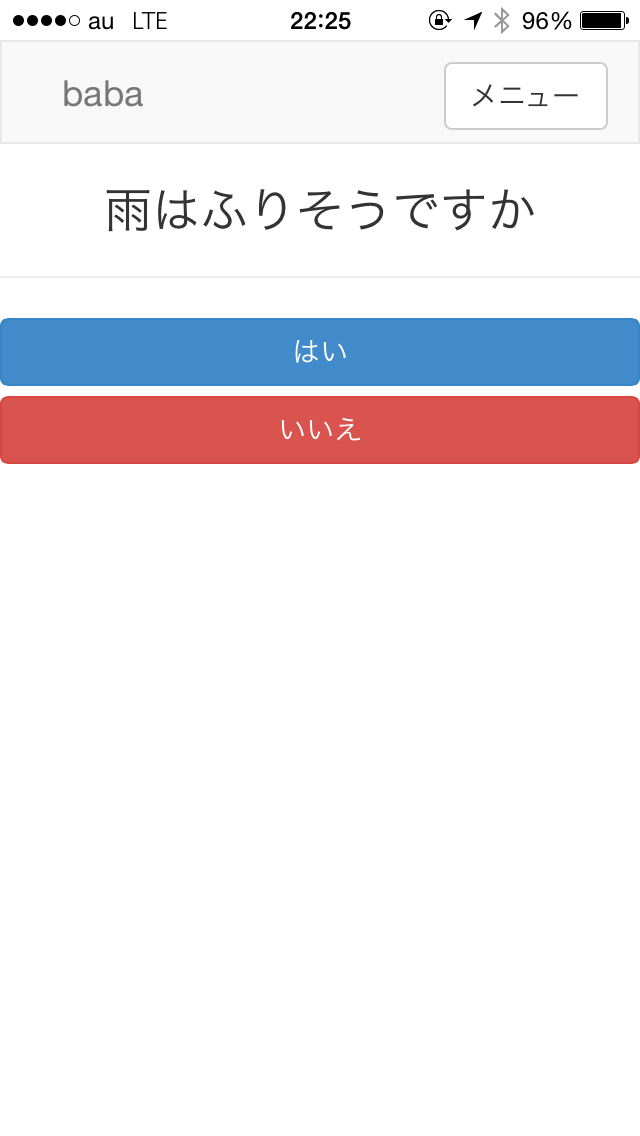
\includegraphics[width=44mm, bb=0 0 640 1136]{images/format_01.png}
  }
  \caption{Babascript Clientインタフェース}
  \label{webapp-interface}
\end{figure}

\section{BabaScript}

Babascriptは、関数呼び出しによって人に処理命令を送る機能に特化したDSL(Domain Specific Language)である。
図\ref{script_01}のようなプログラムによって、人に処理命令を送ることができる。

Babascriptは、シンプルな記法で人力処理のためのプログラムを書けるようにすることを目的としている。

\subsection{基本仕様}

Babascriptでは、定義されていないメソッドが実行されると、エラーを返さずに、人への命令構文として解釈する。
つまり、定義されていないメソッドは全て人への命令として実行され、人へと命令として通知される。
例えば、「toString」や「create」というメソッドは、javascriptにおいてはほぼすべてのオブジェクトが持つメソッドだ。
一方で、「clean\_up\_your\_room」や「bake\_bread」のようなメソッドは定義しない限りは存在しないメソッドだ。
Babascriptは、後者に該当する、定義されていないメソッドをエラーとして評価せず、人への命令構文として評価する。

人への命令構文として評価されたメソッドは、そのメソッド名と引数を元にしたタスク情報を生成し、BabascriptClientへと送信する。

命令の実行結果をBabascriptClientから受け取ると、関数の実行を終了し、指定したコールバック関数が実行される。
コールバック関数実行時には、引数として、処理に成功していれば、処理実行者が入力した結果が、処理失敗であればエラー文が代入されている。
人への処理命令は、通常の関数呼び出しとほぼ同じ記法で実行することができ、新たに記法を学習するといった必要がない。

人オブジェクトは宣言時にIDを指定することによって、誰に対して命令を配信するかを決定する。
例えば、id=baba に命令を送りたければ、人オブジェクト宣言時の第一引数にはbabaという文字列を指定する必要がある。
また、クライアント側でも同様に、id=baba として宣言する必要がある。



% 考えなおし
この際、指定したIDを監視するクライアントが複数人だった場合は、後述するbroadcastオプションをつかってない場合は、
命令を実行していないクライアントへと順番に配信される。

\subsection{オプション情報の付加}
人への命令構文の第一引数には、基本的な情報以外にクライアント側に伝えたい情報を格納したオブジェクトを与える。
例えば、返り値の型を指定などの情報が考えられる。
List型を返り値の型として指定する場合にはプログラム例\ref{script_02}のようなプログラムが考えられる。

% ここも考えなおし
\begin{lstlisting}[caption=オプション情報例(Boolean), label=script_02]
#!/usr/bin/env baba

Babascript = require("babascript");
baba = new Babascript("baba");
sho = new Babascript("sho");
opitons = {
  format: "list"
  list: ["寒い", "普通", "暑い"]
};
baba. 部屋の温度はどうですか(options, function(result){
  if(result.value === "寒い"){
    sho. 部屋の温度を上げてください();
  }else if(result.value === "暑い"){
    sho. 部屋の温度を下げてください();
  }
  process.exit();
});

\end{lstlisting}

% 考えなおし
特別なオプション情報として、broadcastオプションが存在する。
broadcast機能は、指定したIDを監視する全てのクライアントへとタスクを配信し、指定した数の返り値を得られると処理を終了し、コールバック関数を実行するといったものだ。

\section{Babasciript Client}

Babascript Clientは、Babascriptからの命令を受け取り、値を返すためのスマートフォン向けアプリケーションである。
Babascriptとの通信を担うライブラリ部分と、返り値の入力等を担うインタフェース部分から構成される。
両者を分離することによって、インタフェース部分を自由に変更することも可能である。
本論文においてはスマートフォン向けアプリケーションとしてインタフェース部分を実装したが、汎用的な実世界入力インタフェースを利用するといったことも可能だ。

% 様々なアプリケーションに、Babascriptからの命令を受け取って値を返すための機能を組み込めるようにする
% 様々な既存のアプリケーションに人力処理のためのクライアント機能を組み込めるようにすることと、
% 処理実行者にとって、実行するべきことがすぐにわかって、その処理結果をすぐに返せるようにすることを目的としている。
% そのため、命令を受け取る通信を行うためのライブラリ部と、返り値の入力を受け付けるUI部が分離されている。

\subsection{ライブラリ}
ライブラリ部分では、主にBabascriptとの通信をおこなっている。
命令受信のイベントに対してコールバック関数を指定することで、処理命令を受け取ることができる。
基本的な利用方法は、図\ref{client_library}に示す。

\begin{lstlisting}[caption=BabascriptClientのライブラリコード, label=client_library]

// Babascript Clientのライブラリ読み込み
Client = require('babascript-client');
// Clientオブジェクトの宣言
baba = new BabascriptClient("baba");

// 命令を受信すると、 get_task という
// イベントと紐付けられた関数が実行される
baba.on("get_task", function(task){
  // ユーザに命令内容を示す
  $("#task-body").html(task.key);
  $("#true-button").click(function(e){
    // true のボタンが押されたら
    // true を返り値として Babascript に返す
    baba.returnValue(true);
  });
  $("#false-button").click(function(e){
    // false のボタンが押されたら
    // false を返り値として Babascript に返す
    baba.returnValue(false);
  });
});

\end{lstlisting}

クライアントオブジェクトの宣言時、IDを指定することによって、IDに対して処理命令が発行された際にタスクを受信することができる。
また、クライアントオブジェクトが持つreturnValueメソッドを利用することで、返り値を命令発行元に返すことができる。

クライアントライブラリは、UIと完全に分離した実装となっており、かつ利用法もシンプルだ。
後述のWebアプリケーションだけでなく、様々なアプリケーションに組み込むことができる。
既存のアプリケーションであったとしても、数行のコードとインタフェース部分を実装するだけである。

\subsection{Webアプリケーション}

送られてきた命令内容をユーザに提示するためのインタフェースとして、スマートフォン向けWebアプリケーションを実装した。
Babascriptによる命令構文実行時に型指定をしておくことによって、ユーザに提示するインタフェースが変化するようになっている。
インタフェースを変化させることによって、型に合った返り値を選択できるようにしている。
例えば、Boolean型を指定していた場合、ユーザには true ボタンと false ボタンが提示され、どちらかを押すと、その結果が返り値としてプログラムに返される。

% ここの根拠
スマートフォンに最適化したWebアプリケーションとして実装しており、様々な場面において利用可能だ。
実世界におけるタスクを処理しながらでも十分に利用可能である。
図\ref{webapp-interface}のような画面を持つ。

\section{実装}

上記システムは全てJavaScriptで実装した。\\
BabascriptはJavaScriptのサーバサイド実行環境であるNode.js上で動作する。
また、Babascript ClientはWebブラウザ上及びNode.js上で動作する。
全体図は図\ref{system}のとおりだ。

\begin{figure}[h]
  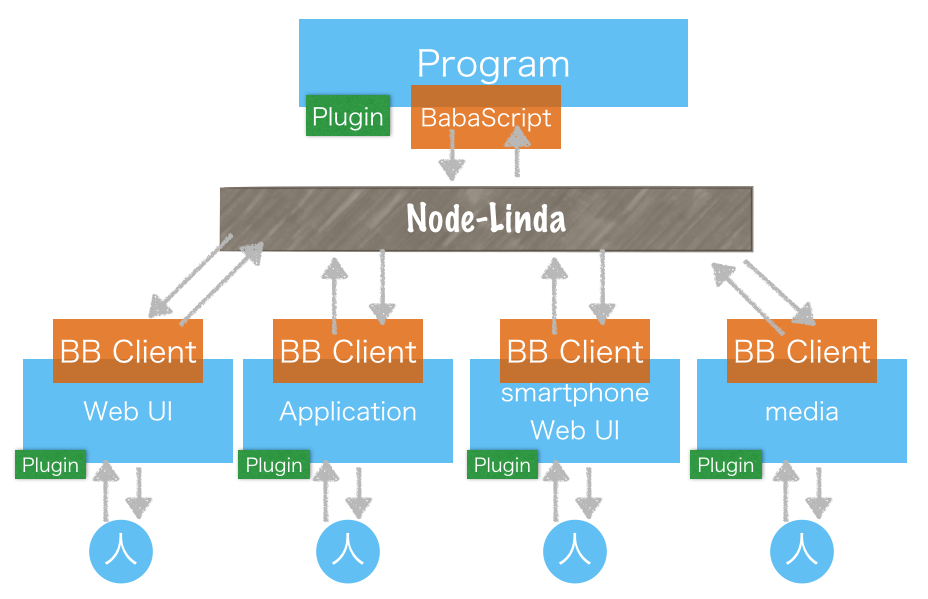
\includegraphics[width=83mm, bb=0 0 928 599]{./images/system.png}
  \caption{システム全体図}  
  \label{system}
\end{figure}

BabascriptとBabascriptClient間の通信を実現するために、Node-Linda\cite{linda}を利用した。

\subsection{処理の流れ}

Babascriptは、以下のような流れで人への命令構文が実行される。

1. 人への命令構文を実行する
2. 命令がNode-Lindaサーバを経由してクライアントへと配信される
3. 命令を受け取ったクライアントがユーザに処理を促す
4. 命令実行者が、処理結果をBabascriptClientに入力する
6. Node-Lindaサーバを経由して実行元プログラムに入力された処理結果が送信される
7. プログラム側で指定されたコールバック関数が実行され、処理が継続される

\subsection{タスク情報の構成}

人への処理命令構文の実行によってタスク情報が生成される。
このタスク情報は、図\ref{task}のようなjsonオブジェクトとなる。

\begin{figure}[!h]
  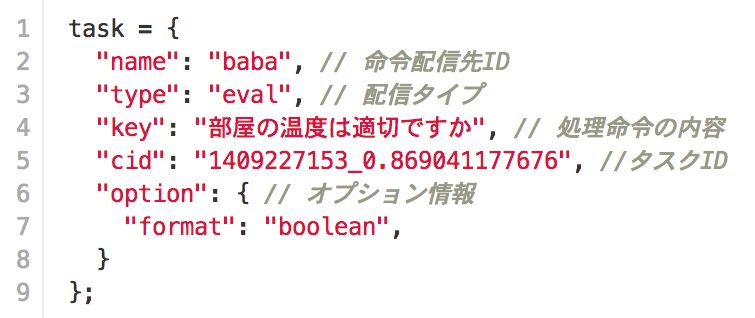
\includegraphics[width=83mm, bb=0 0 755 318]{./images/task.png}
  \caption{タスクのJSONオブジェクト}  
  \label{task}
\end{figure}

\section{応用例}

以下のような応用が考えられる。

\subsection{仕事のプログラム化}
% みでもできてしまい、部分部分で人の意思や感性、知識を加えるだけで良い -->

人への命令がプログラムとして記述可能になることで、人の仕事をプログラム化することができると考える。
人の仕事は、例えば、マニュアルのような形で記述されることが多い。
マニュアルで全て記述できるような場合は、Aという条件の時にはBの処理を実行する、といったことが文章として記述されていることが多く、その内容の多くはプログラムのようなものであるため、プログラム化は可能であると言える。

プログラム化し、実行することによって、状態をプログラムによって管理することが可能となる。
つまり、条件判断や記憶が必要なことは出来るだけコンピュータ側に処理させる、といったことが可能になる。
人は細かい条件などを覚えておいたり、自分で判断することなく、ただ指示されたことのみを実行することで、仕事を終わらせることができるようになる。
ただ指示されたことのみを実行するだけで良いならば、仕事の引き継ぎなども必要なくなり、人の代替も容易となる。

また、人同士がコミュニケーションを取ることなく、複数人を協調させるといったことも可能となる。
通常、複数人を協調させるためには、人同士が相談したり、上位の意思決定者が必要となる。
しかし、コミュニケーションはコストのかかるものであり、適切に行われない場合、問題が生じることもある。
意思決定をプログラムに委ねることは、複数人を効率よく協調させることに繋がるとも考えられる。

全ての仕事をプログラム経由にすることで、詳細な実行ログや実行状況を把握することもできる。
仕事の実行量の定量化や、状況監視、状況の可視化などに活かすことができる。

% 具体的なプログラム例

\subsection{人力による実世界プログラミング}

人をセンサーやアクチュエータとして利用することで、人を使って実世界を操作する、人力実世界プログラミングが可能となる。
現在のセンサーやアクチュエータでは、実世界に干渉するのには限界がある。
例えば、その場の雰囲気を数値化したり文字列化するといった、コンテキスト情報を伴ったセンシングは困難である。
しかし、人力処理を組み込むことのできる本提案手法ならば、コンテキスト情報を伴うようなセンシングであっても、実現可能である。
また、人を汎用的に利用可能なアクチュエータとして利用することもできる。

人をセンサーとして扱う手法は、Human as Sensorと呼ばれ、研究が多く存在しているが、人をアクチュエータとして利用する、Human as Actuator と言えるような事例は少ない。
両者を組み合わせることによって、より柔軟に実世界へと干渉可能なプログラミングが可能となる。

また、本提案手法では通常のプログラムと人力処理のプログラムを混合させることができるため、
条件次第で人とコンピュータのどちらに処理させるかをプログラムが判断し、適切な方に処理させるということも可能である。

% 具体的なプログラム例

\section{考察}

Babascriptについて、以下のように考察する。

\subsection{処理に対する人の積極的な貢献}

プログラムは、コンピュータの能力を利用して人を支援するためのものであり、人はその恩恵を得るのみであった。
コンピュータで実行可能であるならば、コンピュータで実行するのが良い。
しかし、人にしか出来ないことも現在の技術では存在する。
そこで処理の実現を諦めるのではなく、コンピュータが得意なことはコンピュータが、人が得意なことは人がやるようにすれば良い。
人が積極的に処理に貢献することによって、全体的な処理の正確性の向上や高速化に寄与する可能性も存在する。
それはまた、人にとってもメリットになりうるのではないかと考える。

\subsection{処理単位としての人}

本研究では、人は処理を命令され実行するノードとなり、プログラム上においてコンピュータやセンサーと同等となる。
こういったことに対して心理的な拒否感を覚えることも考えられる。
しかし、一処理ノードとして扱うことは、大きなメリットでもある。
命令を実行するだけのノードであるということは、ただ処理内容を実行することにのみ集中すれば良いということだ。
ただやるべきことだけが提示され、その通りに動けば良いということは、深く考える必要がなく、楽であるということが考えられる。
もちろん、全ての処理がただ提示する通りに動けば良いものではないと考えられるが、
作業を楽にするための一つのアイデアであると言える。

\subsection{タスク実行の遅延と実行保障性}

Babascriptによってタスク実行を依頼しても、人がすぐにタスクを実行し値を返すことを完全に保証することはできない。
タスク受信端末を見ていない、受信しても実行できないといった状況の場合、すぐに値を返すことはできない。
この際、Babascriptによる処理が原因で全体の処理が遅延する可能性がある。

また、労働関係にあるなど、タスク実行に強制力がある場合は、タスク実行が確実に行われると考えられるが、強制力がない場合はそもそもタスク受信を無視するといったことも考えられる。
タスク実行に強制力がない場合は、金銭などのインセンティブを与えるといった手段によって、実行保障性を確保するといったことが考えられる。

\subsection{例外処理}

Babascriptにおいて、命令が想定する状況と現実の状況との乖離によって適切な返り値を選択・記述ができなくなるといった可能性がある。
これは、現実が刻々と変化していることなどから、完全に避ける事の出来ない問題であると考える。
この際、無理やり値を返すといった処理をしてしまうと、本来の状態とは違った判断がなされてしまう危険性がある。
命令文とは明らかに現実が異なっている場合などは、タスク実行者から例外としてプログラムに通知出来るような仕組みの実装によって、問題の解決へと繋げられると考える。

\subsection{命令内容の粒度}

Babascriptでは、タスクの命令文の記述には制限がない。
そのため、命令の抽象度はプログラムを書く人に依存する。
抽象度が高すぎる命令文にしてしまうと、タスク実行者にとって理解しづらい文面となり得る。
例えば、「アレをする」といったような命令文の場合、タスク実行者は命令内容を理解できないと考えられる。
その結果、想定外の処理が実行され、意図しない結果を招く恐れがある。

具体的過ぎる命令は、全体の処理内容にもよるが、プログラム自体が冗長となり得る。
例えば、...? % TODO ここなおす!!
プログラムとタスク実行者の間のやりとりが増え、通信や待機時間などがボトルネックとなる可能性がある。
また、タスク実行者にとっても、やりとりが増えることで負担増になると考えられる。

処理ごとに異なると考えられるが、命令文は適切な抽象度に設計しなくてはならない。

\subsection{複数命令の同時実行}

複数のプログラムから同時に一人のタスク実行者へとタスクが配信される可能性がある。
この際、異なるコンテキストにある命令が交互に配信され、タスク実行に大きな障害をもたらす可能性がある。
例えば、料理プログラムと掃除プログラムが同時に実行された場合、鍋で煮ている途中に「洗剤を投入しろ」などといった命令が配信されることが考えられる。

この問題は、全てのBabascriptプログラム中において、一人のタスク実行者は一つのプログラムからのみ、連続してタスクを受信できるような仕組みを用意することによって、解決可能であると考えられる。
また、応用アプリケーションでの実装になるが、コンテキストを明示し、どの処理系におけるタスクなのかをタスク実行者に示すといった手段によっても解決可能である。

\section{関連研究}

計算機では処理が難しいようなタスクを解決するために、人を計算資源として利用する手法はヒューマンコンピュテーション\cite{humancomputation}と呼ばれ、様々な研究が行われている。
インターネットを介して不特定多数の群衆にタスクを実行させるクラウドソーシングと組み合わせた研究事例も多く存在する。

クラウドソーシングのプラットフォームとしては、Amazon Mechanical Turk\cite{mechanicalturk}が存在する。
Barowy らは、CrowdProgrammingという概念を提唱し、プログラミング言語内においてクラウドソーシングによる計算とコンピュータによる計算の統合を実現した\cite{automan}。
Franklin らは、機械だけでは答えられないようなDBへのクエリに対する応答を、クラウドソーシングを用いることで返答可能にするCrowdDBを提案している\cite{crowddb}。
Morishima らは、人をデータソースとしてプログラムの中で利用する手法を提案している\cite{cylog}。
これらの研究では、クラウドソーシングを利用した問題解決手法の提案をしている。
本研究は、不特定多数の群衆をプログラムするためのものではなく、実世界の操作なども含むため、家族や職場の人のような特定可能な人物を対象としている。
また、人を計算資源やデータソースとしてシステムに組み込むことを前提としているが、本研究は、計算資源やデータソースに限らず、実世界への干渉等も対象としている。
本研究はより汎用的な枠組みであると言える。

% TODO 直せ
Ahmad らは、Jabberwocky\cite{jabberwocky}という、Dormouse・ManReduce・Dogの3要素から成るソーシャルコンピューティングのための一連の仕組みを提案している。
また、Dog\cite{dog}というWebアプリケーションにおけるユーザとのインタラクションを。。。?


% Ahmad らは、Dogという独自のプログラミング言語を提案している。
% Dogは、Webアプリケーションにおけるユーザとのインタラクションを

ユビキタスコンピューティングの研究分野においては、Human as Sensorという、人や人が持つスマートフォンをセンサーとして利用する概念も提唱されている。
PRISMは、スマートフォンを利用したセンシングプラットフォームだ\cite{prism}。
Liuらは、ソーシャルメディア上の人をセンサーとして扱ったQ\&AサービスMoboQを提案し、その検証を行った。
Human as Sensorに類する研究では、人をセンサーとして扱うことを対象としているが、本研究ではセンサーのみを対象としていない。

Chengらは、モーションプラットフォームにおけるモーターやメカニカル機構の代替として人を利用したHaptic Turkを提案している\cite{hapticturk}。
Haptic Turkはゲームでの利用に特化したものだ。
本研究は、用途を限らない汎用的な仕組みとなっている。

加藤らは、人とロボット間でのタスク共有システム Sharedoを提案した\cite{sharedo}。
人とロボットのタスク実行における協調についても述べられており、本研究で目的としている
「処理実行において人とコンピュータは協調すべき」という考えと類似している。


\section{おわりに}

本論文では、プログラムに人への処理命令を組み込むことのできるプログラミング環境 Babascript を提案した。
既存の仕組みでは、プログラムから人に処理命令を送るためには、クラウドソーシングプラットフォームが必要であったり、複雑な構文の実行が必要である。
本論文の手法では、身近な特定の人物を命令実行対象とし、よりシンプルな記法で人への処理命令を実現した。
% Babascriptでは、クラウドソーシングを利用せず、シンプルな記法で

また、Babascriptによって実現が見込まれる応用例について言及した。
仕事がプログラム化でき、ただ命令に従うだけで仕事を実行できるようになれば、
人の代替が容易になったり、コンピュータと人が協調してより効率的になると考えられる。

今後の展望としては、考察で述べたBabascriptの問題点についてシステムの改良などを行う。

{\scriptsize
\bibliographystyle{jwiss}
\bibliography{paper}
}

\end{document}


